\documentclass{article}
\usepackage{graphicx}
\usepackage{caption}
\usepackage{subcaption}
\usepackage{hyperref}
\graphicspath{{./figs/}}{}
\usepackage{listings}
\title{
HLS-Assignment 8
}
\begin{document}
\maketitle
\hfill \textbf{Sampath Govardhan} \\
\null \hfill \textbf{FWC22071}\\
\maketitle
\hfill \textbf{VITIS-HLS}
\section{Problem Statement}
\begin{lstlisting}
1. Write an HLS module, along with testbench, for Cyclic Prefix 
removal from an incoming set of data inputs.

2. After HLS testing using HLS testbench and synthesis of the 
module in HLS, export the module to Vivado application.

3. The input to the CP removal module should be given from another 
HLS module which will act as a data generator. Use an array to
store the input values from the attached data set file in the 
mail and perform synthesis in HLS to get the data generator module.

4. Interface both the modules with Xilinx FFT IP and perform FFT
on the output of Cyclic Prefix Removal in the Vivado application.

5. Generate a wrapper for the block diagram in Vivado and then write 
a test bench in Verilog which will provide clock and reset to these 
modules and store the FFT output in a file.

6. Run simulation. Compare the output obtained from Verilog by writing 
a code in MATLAB for the same functionality and check for correctness.

\end{lstlisting}
\vspace{6cm}
\section{Header File}
\begin{lstlisting}
#ifndef _HEADER_H_
#define _HEADER_H_

#include <iostream>
#include <complex>
#include <fstream>
#include <hls_stream.h>
#include <vector>
using namespace std;
#define N 8800
#define P 608   //(320+288)

typedef struct {
    float real;
    float imag;
} ComplexT;

void gen(hls::stream<ComplexT> &gst);
void cyclicPrefixRemoval(hls::stream<ComplexT> &inpstream, hls::stream<ComplexT> &oupstream, hls::stream<bool> &z);

#endif


\end{lstlisting}
\vspace{6cm}

\section{Data Generator Code}
\begin{lstlisting}
#include "header.h"

void gen(hls::stream<ComplexT> &gst) {
#pragma HLS INTERFACE mode=axis register_mode=both port=gst register


value z[N]={{0.36492,-0.728851},{-0.752842,0.31251},{0.875913,0.27137},{-0.36993,-0.787211},{-0.284297,0.793227},{0.106226,0.592726},{0.244906,-0.620938},{-0.559632,0.220519},{0.5804,0.133315},{-0.319342,-0.420631}};

	  for (int i = 0; i < N; i++) {
#pragma HLS PIPELINE II=1
        gst.write(z[i]);

    }
}

\end{lstlisting}
\vspace{15cm}
\section{Cyclic Prefix Removal Code}
\begin{lstlisting}


#include "header.h"

void cyclicPrefixRemoval(hls::stream<ComplexT> &inpstream,
 hls::stream<ComplexT> &oupstream, hls::stream<bool> &z) {
#pragma HLS INTERFACE mode=axis register_mode=off port=z
#pragma HLS INTERFACE mode=axis register_mode=both port=oupstream register
#pragma HLS INTERFACE mode=axis register_mode=both port=inpstream register

ComplexT invar;
ComplexT x[N];
bool last=false;
for (int i=0;i<N;i++){
#pragma HLS PIPELINE II=1
    invar = inpstream.read();
    x[i]=invar;
}
    for(int i=0;i<N-P;i++){
#pragma HLS PIPELINE II=1
    	if(i<4096){
        oupstream.write(x[i+320]);
    	}
    	else{
    	oupstream.write(x[i+608]);
    	if (i == (N - P - 1)) {
    	    	            last = true;
    	    	        }
    	else{last=false;}
    	}

    }
z.write(last);
}


\end{lstlisting}
\vspace{3cm}

\section{Test Bench Code}
\begin{lstlisting}
#include "header.h"

int main() {

    //PART-1:  Taking input values from given .txt files and
	//         storing resultant complex value in an array 
	        // and also in another file.

    ComplexT x[N];
    float c, d;
    float a,b;
    ifstream in1("puschTxAfterChannelReal.txt");
    ifstream in2("puschTxAfterChannelImag.txt");
    //ofstream ival("ival.dat");
    ofstream inp("input.dat");
    int l=0;
    for (int i = 0; i < N; i++) {
    	l=l+1;
        in1 >> c;
        in2 >> d;
        a=c;b=d;
        x[i].real = a;
        x[i].imag=b;
        inp<<"{"<<x[i].real<<","<<x[i].imag<<"}"<<","<<endl;

       /* ival <<"ComplexT"<< x[i-1]<<",";
       if(l%5==0){
    	   ival<<endl;
       }*/
    }

    in1.close();
    in2.close();
    inp.close();

    //PART-2:  The output of CPR is strored in another
            // array and also in another file.

    ofstream oup("output.dat");
    ComplexT y[N];
    hls::stream<ComplexT> gst,oput;
    int t=0;
     hls::stream<bool> bf;
    hls::stream<int> z;
    ComplexT output;

    gen(gst);
    cyclicPrefixRemoval(gst, oput, bf);
        for (int i=0;i<N-P;i++){
        if (!oput.empty()) {
          output = oput.read();
          y[i].real=output.real;
          y[i].imag=output.imag;
          oup<<"{"<<y[i].real<<","<<y[i].imag<<"}"<<","<<endl;
        }
        /*else {
         cout<<"Skipping Cyclic Prefix BITS"<<endl;
       }*/
    }
    oup.close();

    //PART-3:  The input and output values are compared 
    //         using given precision and
    //         then the result is stored in another file

    ofstream out("out.dat");
    int q=0;
    bool f=0;
    for (int i = 0; i < N-P; i++) {
    	q=q+1;
        out << "Output[" << i << "]: " <<
        "{"<<y[i].real<<","<<y[i].imag<<"}"<<"\t";
        if (q<=4096){
        	out<<"FIRST SYMBOL"<<"\t";

        if ((y[i].real-x[i+320].real)/y[i].real < 10e-3 && (y[i].imag
        x[i+320].imag)/y[i].imag <10e-3){
        	out<<"Pass"<<endl;
        }
        else{
        	f=1;
        	//cout<<f<<endl;
        	out<<"Fail"<<endl;
        }
    }
    else{
    	out<<"SECOND SYMBOL"<<"\t";
        if ((y[i].real-x[i+P].real)/y[i].real < 10e-3 && (y[i].imag
        x[i+P].imag)y[i].imag < 10e-3){
        	out<<"Pass"<<endl;
        }
        else{
        	f=1;
        	//cout<<f<<endl;
        out<<"Fail"<<endl;
        }
    }
    }
    out.close();
    if (f==1){cout<<"!!FAIL!! OUTPUT IS NOT TOLERABLE BASED ON GIVEN
    PRECISION"<<endl;}
    else {cout<<"!PASS! OUTPUT IS TOLERABLE BASED ON GIVEN 
    PRECISION"<<endl;}
    return 0;

}

\end{lstlisting}
\vspace{3cm}


\section{C simulation Output}
\begin{lstlisting}
INFO: [SIM 2] *************** CSIM start ***************
INFO: [SIM 4] CSIM will launch GCC as the compiler.
make: 'csim.exe' is up to date.
!PASS! OUTPUT IS TOLERABLE BASED ON GIVEN PRECISION
WARNING [HLS SIM]: hls::stream 'hls::stream<bool, 0>0' contains 
leftover data, which may result in RTL simulation hanging.
INFO [HLS SIM]: The maximum depth reached by any hls::stream() 
instance in the design is 8800
INFO: [SIM 1] CSim done with 0 errors.
INFO: [SIM 3] *************** CSIM finish ***************




\end{lstlisting}
\vspace{10cm}



\section{HLS Resource Consumption}
\vspace{1cm}
\begin{figure}[h]
\centering
\begin{subfigure}{0.6\textwidth}
    \centering
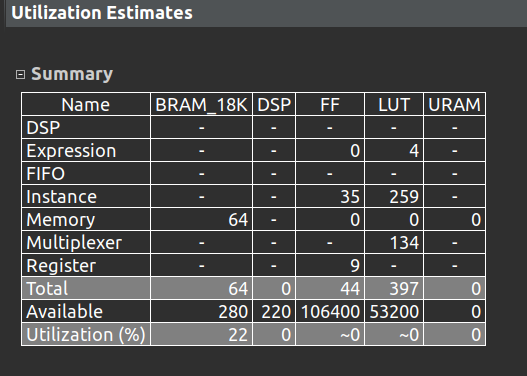
\includegraphics[width=\textwidth]{figs/cpr1.png}
    \caption{CP Removal}
    \label{fig:my_label}
\end{subfigure}
\hfill
\begin{subfigure}{0.6\textwidth}
    \centering
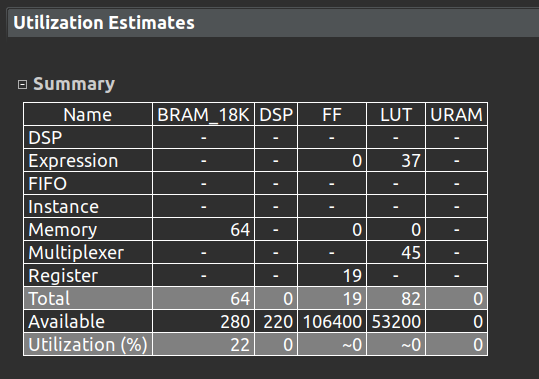
\includegraphics[width=\textwidth]{figs/gen1.png}
    \caption{Generator}
    \label{fig:my_label}
\end{subfigure}
\end{figure}

\vspace{3cm}


\section{HLS Timing Report}
\vspace{1cm}
\begin{figure}[h]
\centering
\begin{subfigure}[b]{0.5\textwidth}
    \centering
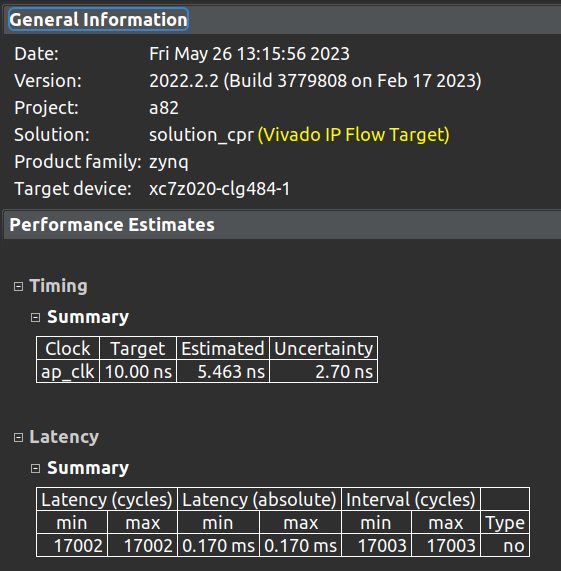
\includegraphics[width=\textwidth]{figs/cpr2.png}
    \caption{CP Removal}
    \label{fig:my_label}
\end{subfigure}
\hfill
\begin{subfigure}[b]{0.5\textwidth}
    \centering
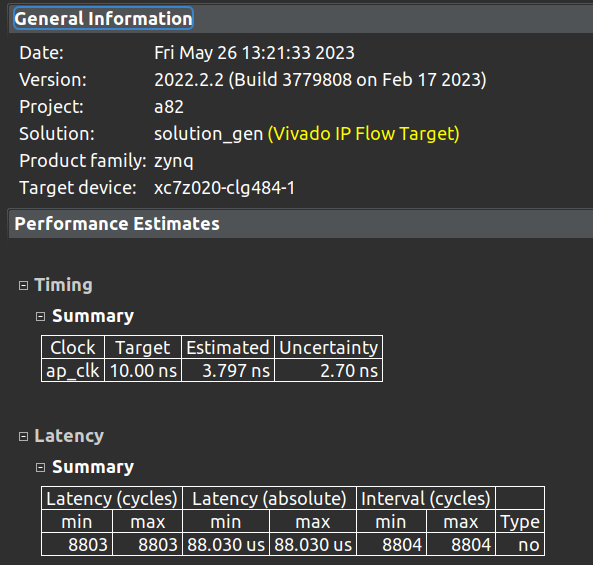
\includegraphics[width=\textwidth]{figs/gen2.png}
    \caption{Generator}
    \label{fig:my_label}
\end{subfigure}
\end{figure}

\vspace{15cm}


\section{CoSimulation Report}
\vspace{1cm}
\begin{figure}[h]
\centering
\begin{subfigure}[b]{1.2\textwidth}
    \centering
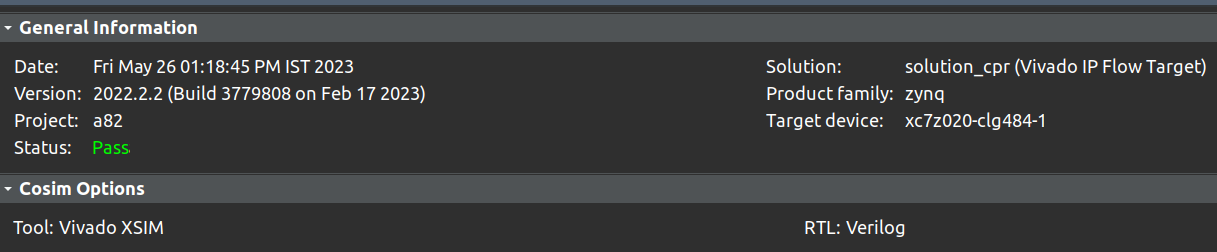
\includegraphics[width=\textwidth]{figs/cpr3.png}
    \caption{CP Removal}
    \label{fig:my_label}
\end{subfigure}
\hfill
\begin{subfigure}[b]{1.2\textwidth}
    \centering
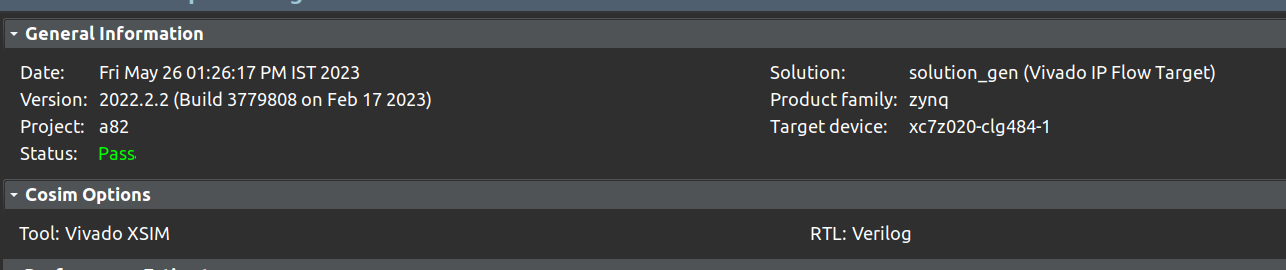
\includegraphics[width=\textwidth]{figs/gen3.png}
    \caption{Generator}
    \label{fig:my_label}
\end{subfigure}
\end{figure}
\vspace{15cm}


\maketitle
\hfill \textbf{VIVADO}
\section{Block Design}
\vspace{1cm}
\begin{figure}[h]
    \centering
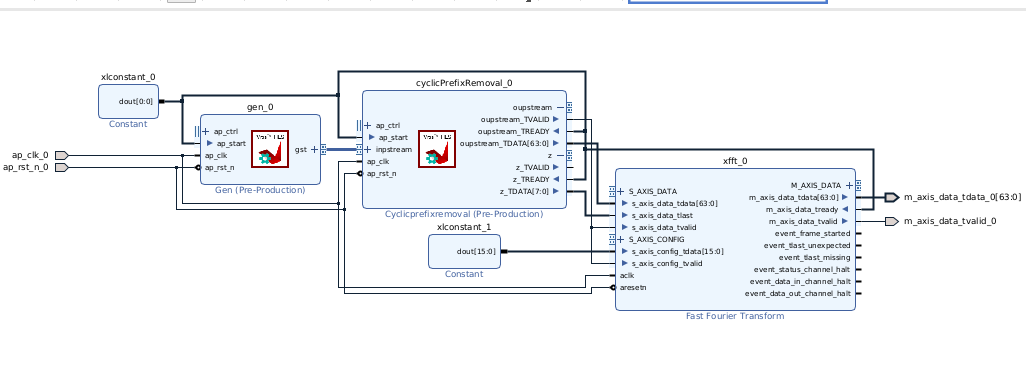
\includegraphics[width=\columnwidth]{figs/bd.png}
    \caption{Cosimulation Report}
    \label{fig:my_label}
\end{figure}
\vspace{3cm}
\section{Verilog Testbench}
\begin{lstlisting}
// Engineer: 
// 
// Create Date: 05/25/2023 11:59:07 AM
// Design Name: 
// Module Name: wav_tb
// Project Name: 
// Target Devices: 
// Tool Versions: 
// Description: 
// 
// Dependencies: 
// 
// Revision:
// Revision 0.01 - File Created
// Additional Comments:
// 
//////////////////////////////////////////////////////////////////////////////////


module wav_tb(

    );
    
  reg clk; 
  reg rst;
  wire [63:0]m_axis_data_tdata_0;
  wire m_axis_data_tvalid_0;
  integer file;
  reg [31:0] sample_counter;

  design_1_wrapper i
       (.ap_clk_0(clk),
        .ap_rst_n_0(rst),
        .m_axis_data_tdata_0(m_axis_data_tdata_0),
        .m_axis_data_tvalid_0(m_axis_data_tvalid_0));
        

                                       
        always #5 clk=~clk;
        initial begin
        
        rst=0;clk=1;
        #100 rst=1;
        #89130000 $finish;
        end      
        
        initial begin
        
        file=$fopen("fft_output_vivadoip.txt","w");
        sample_counter = 0;

    while (sample_counter < 8192) begin
      #10;  // Assuming a sampling rate of 10 units

        if (m_axis_data_tvalid_0) begin
         $fwrite(file, "%h\n", m_axis_data_tdata_0);
        sample_counter = sample_counter + 1;
      end
    end

    $fclose(file);
  end
endmodule

\end{lstlisting}

\vspace{3cm}


\section{Output Waveform}
\vspace{1cm}
\begin{figure}[h]
\centering
\begin{subfigure}[b]{1.2\textwidth}
    \centering
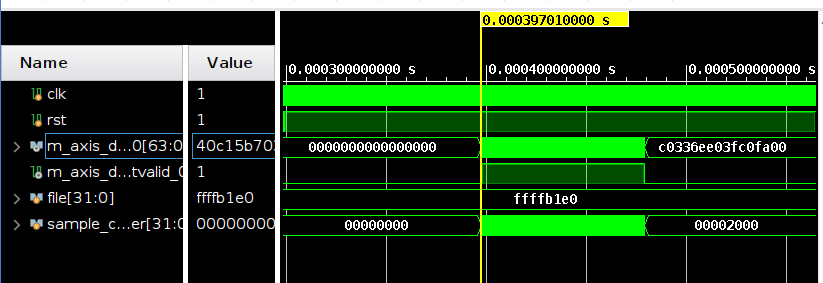
\includegraphics[width=\textwidth]{figs/wav1.png}
    \caption{output of FFT}
    \label{fig:my_label}
\end{subfigure}
\hfill
\begin{subfigure}[b]{1.2\textwidth}
    \centering
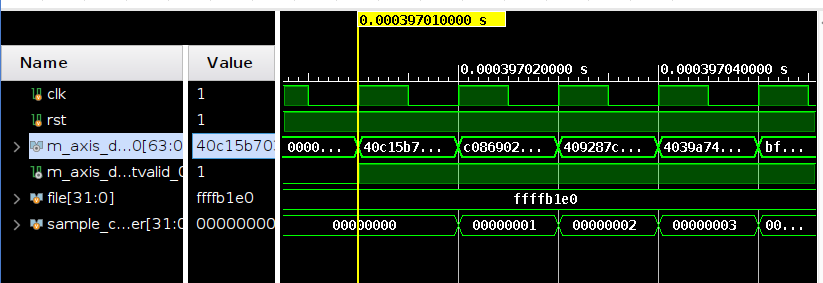
\includegraphics[width=\textwidth]{figs/wav2.png}
    \caption{Zoomed format of above figure}
    \label{fig:my_label}
\end{subfigure}
\end{figure}
\vspace{15cm}

\maketitle
\hfill \textbf{MATLAB}
\section{Matlab Code}
\begin{lstlisting}
clc;
close all;
x = [complex(-0.601084,-0.059909) complex(0.571592,0.530777) complex(0.096652,-0.704768) complex(-0.493203,0.428746) 
X = fft(x);

disp('FFT Output:');
disp(X);

fileID = fopen('fft_output_matlab.txt', 'w');
fprintf(fileID, 'Real \t Imaginary \n');
for k = 1:length(X)
    fprintf(fileID, '%d \t %d \n', real(X(k)), imag(X(k)));
end
fclose(fileID);

\end{lstlisting}
\vspace{3cm}
\section{Conclusion}
\begin{lstlisting}
The Output of FFTIP is matching with Output of Matlab with Precision 
using this floating Point Converter Online :

\end{lstlisting}
\url{https://www.h-schmidt.net/FloatConverter/IEEE754.html}
\vspace{4cm}
\\
\textbf{GITHUB :} \url{https://github.com/dk-425/Training.git}
\end{document}


